%if printing on both sides of a page add 'twopage' to the [...] below
\documentclass[11pt,openright]{report} 
\usepackage{graphicx}
\usepackage{color}
\usepackage{tocbibind}
%\usepackage{algorithm2e} % must be included before unlv-thesis
\usepackage[linesnumbered,ruled]{algorithm2e}
\SetKwProg{Fn}{Function}{}{}
\usepackage{subcaption}
\usepackage{fancyhdr}
\usepackage{unlv-thesis}

\graphicspath{{./images/}, {./results/}}
\usepackage{hyperref}
\hypersetup{
	colorlinks=false, %set true if you want colored links
	linktoc=all,     %set to all if you want both sections and subsections linked
	linkcolor=blue,  %choose some color if you want links to stand out
}
%%%
%%% Choose either \phdthesis or \mastersthesis
\mastersthesis
%\phdthesis

%%%
%%% opens all chapters on right hand sides (needed for double sided printing)
\leftchapter
%%% add \twosided if you are printing on both sides
%\twosided
%%%
%%% Choose the spacing for the thesis: \singlespace, \oneandhalfspace or \doublespace
%\oneandhalfspace
%\singlespace
\doublespace

\makeindex

%%%
%%% The name of your thesis and your own name. Title must be in all
%%% caps and in an inverted triangle
\thesistitle{SECURE DECENTRALIZED STORAGE USING BLOCKCHAIN}
\thesistitlelowercase{Secure Decentralized Storage Using Blockchain}
\thesisauthor{Vinay Kumar Calastry Ramesh}

%%%
%%% Add your previous degrees here
\thesisauthorpreviousdegrees{
Bachelor of Technology in Computer Science\\ \vspace*{-0.12in}
Jawaharlal Nehru Technological University, Hyderabad\\ \vspace*{-0.12in}
2014}

%%%
%%% Month and Year to appear on the thesis
\thesismonth{May} 
\thesisyear{2019}
\copyrightyear{2019}

%%%
%%% The size of the committee: chair + other members + college rep (normally 4)
%%% use \chair{}, \memberone{}, \membertwo{}, \memberthree{}, \colleferep{}
\thesiscommitteesize{4}
%\signatures{}   % will generate 'signatures on the approval page' grad college does 
%not like this, so don't do that in their version
\chair{Yoohwan\ Kim, Ph.D.}
\memberone{Laxmi\ Gewali, Ph.D.}
\membertwo{Fatma\ Nasoz, Ph.D.}
\collegerep{Ge\ Lin\ Kan, Ph.D.}

%----------------------- Macros ----------------------------------------- 

%\newcounter{defcounter}
%\setcounter{defcounter}{1}
%\newcounter{excounter}
%\setcounter{excounter}{1}
%\newcounter{propcounter}
%\setcounter{propcounter}{1}
%\newcounter{lemmacounter}
%\setcounter{lemmacounter}{1}
%\newcounter{theoremcounter}
%\setcounter{theoremcounter}{1}                    
\newcommand{\mytheoremcounter}{section}
\newcommand{\cheapHack}{ }
\newcommand{\BAPrn}{BAP$_{\mbox{r}}$}
\newcommand{\BAPr}{BAP$_{\mbox{r}}$\ }
\newcommand{\BAPsn}{BAP$_{\mbox{s}}$}
\newcommand{\BAPs}{BAP$_{\mbox{s}}$\ }
\newcommand{\BAPsrn}{BAP$_{\mbox{sr}}$}
\newcommand{\BAPsr}{BAP$_{\mbox{sr}}$\ }
\newcommand{\BAPucn}{BAP$_{\mbox{sr}}$}
\newcommand{\BAPuc}{BAP$_{\mbox{sr}}$\ }
\newcommand{\BSPrn}{BSP$_{\mbox{r}}$}
\newcommand{\BSPr}{BSP$_{\mbox{r}}$\ }
\newcommand{\BSPsn}{BSP$_{\mbox{s}}$}
\newcommand{\BSPs}{BSP$_{\mbox{s}}$\ }
\newcommand{\BSPsrn}{BSP$_{\mbox{sr}}$}
\newcommand{\BSPsr}{BSP$_{\mbox{sr}}$\ }
\newcommand{\BSPucn}{BSP$_{\mbox{sr}}$}
\newcommand{\BSPuc}{BSP$_{\mbox{sr}}$\ }
\newcommand{\NBAPrn}{NBAP$_{\mbox{r}}$}
\newcommand{\NBAPr}{NBAP$_{\mbox{r}}$\ }
\newcommand{\NBAPsn}{NBAP$_{\mbox{s}}$}
\newcommand{\NBAPs}{NBAP$_{\mbox{s}}$\ }
\newcommand{\NBAPsrn}{NBAP$_{\mbox{sr}}$}
\newcommand{\NBAPsr}{NBAP$_{\mbox{sr}}$\ }
\newcommand{\NBAPucn}{NBAP$_{\mbox{sr}}$}
\newcommand{\NBAPuc}{NBAP$_{\mbox{sr}}$\ }
\newcommand{\fixme}[1]{$\spadesuit$\marginpar{\tiny$\spadesuit$#1}}
\newcommand{\Xhalf}{X_\frac{1}{2}}
\newcommand{\Shalf}{\cS_{\frac{n}{2},n}}
\newcommand{\chih}{\chi_n}
\newcommand{\notchih}{\overline{\chi_n}}
\newcommand{\upsh}{\upsilon_n}
\newcommand{\notupsh}{\overline{\upsilon_n}}
\newcommand{\singlespacing}{\baselineskip 1em}
\newcommand{\onehalfspacing}{\baselineskip 1.25em}
\newcommand{\doublespacing}{\baselineskip 1.75em}
\newcommand{\truedoublespacing}{\baselineskip 2em}
\newcommand{\normalspacing}{\singlespacing}
\newcommand{\Paccept}[1]{{\Pr[#1 = \mathrm{accept}]}}
\newcommand{\Maj}{\mathit{Maj}}
\newcommand{\Nand}{\uparrow}
\newcommand{\Nor}{\downarrow}
\newcommand{\myem}[1]{{\bf #1}}
\newcommand{\reccr}[1]{\overline{\nu}(#1)}
\newcommand{\regcr}[1]{\nu(#1)}
\newcommand{\LOGDCFLclass}{\mathbf{LOGDCFL}}
\newcommand{\NLclass}{\mathbf{NL}}
\newcommand{\ACclass}{\mathbf{AC}}
\newcommand{\NCclass}{\mathbf{NC}}
\newcommand{\SCclass}{\mathbf{SC}}
\newcommand{\RCclass}{\mathbf{RC}}
\newcommand{\coNLclass}{\mathbf{co\!-\!NL}}
\newcommand{\Lclass}{\mathbf{L}}
\newcommand{\Lpoly}{\mathbf{L}_{/\mathrm{poly}}}
\newcommand{\Pclass}{\mathbf{P}}
\newcommand{\BPclass}{\mathbf{P}_{BP}}
\newcommand{\BPwidth}[1]{\mathbf{P}_{BP}^{#1}}
\newcommand{\NPclass}{\mathbf{NP}}
\newcommand{\coNPclass}{\mathbf{coNP}}
\newcommand{\PPclass}{\mathbf{PP}}
\newcommand{\BPPclass}{\mathbf{BPP}}
\newcommand{\ZPPclass}{\mathbf{ZPP}}
\newcommand{\RPclass}{\mathbf{RP}}
\newcommand{\coRPclass}{\mathbf{co\!-\!RP}}
\newcommand{\SigmaP}[1]{\mathbf{\Sigma_{#1}P}}
\newcommand{\PHclass}{\mathbf{PH}}
\newcommand{\PSPACE}{\mathbf{PSPACE}}
\newcommand{\RSPACE}{\mathbf{RSPACE}}
\newcommand{\DSPACE}{\mathbf{DSPACE}}
\newcommand{\imin}{{\mathit{min}}}
\newcommand{\imax}{{\mathit{max}}}
\newcommand{\gbf}{{\mathbf{g}}}
\newcommand{\zbf}{{\mathbf{z}}}
\newcommand{\wbf}{{\mathbf{w}}}
\newcommand{\vbf}{{\mathbf{v}}}
\newcommand{\xbf}{{\mathbf{v}}}
\newcommand{\onebf}{{\mathbf{1}}}
\newcommand{\zerobf}{{\mathbf{0}}}
\newcommand{\uvec}{\vec{u}}
\newcommand{\vvec}{\vec{v}}
\newcommand{\xvec}{\vec{x}}
\newcommand{\Deltap}{\Delta^\prime}
\newcommand{\Sigmap}{{\Sigma^\prime}}
\newcommand{\alphap}{\alpha^\prime}
\newcommand{\betap}{\beta^\prime}
\newcommand{\betapp}{\beta^{\prime\prime}}
\newcommand{\gammap}{\gamma^\prime}
\newcommand{\mup}{\mu^\prime}
\newcommand{\mupp}{\mu^{\prime\prime}}
\newcommand{\nubar}{{\overline{\nu}}}
\newcommand{\nubars}{\nubar^*}
\newcommand{\nus}{\nu^*}
\newcommand{\betas}{\beta^*}
\newcommand{\deltas}{\delta^*}
\newcommand{\deltap}{\delta^\prime}
\newcommand{\deltapp}{\delta^{\prime\prime}}
\newcommand{\lambdabar}{\overline{\lambda}}
\newcommand{\lambdap}{\lambda^\prime}
\newcommand{\lambdapp}{\lambda^{\prime\prime}}
\newcommand{\pip}{\pi^\prime}
\newcommand{\pipp}{{\pi^{\prime\prime}}}
\newcommand{\Psip}{\Psi^\prime}
\newcommand{\psip}{\psi^\prime}
\newcommand{\phip}{\phi^\prime}
\newcommand{\sigmap}{\sigma^\prime}
\newcommand{\etap}{\eta^\prime}
\newcommand{\etapp}{{\eta^{\prime\prime}}}
\newcommand{\epsilonp}{{\epsilon^\prime}}
\newcommand{\epsilonpp}{\epsilon^{\prime\prime}}
\newcommand{\epsilonppp}{\epsilon^{\prime\prime\prime}}
\newcommand{\ap}{a^\prime}
\newcommand{\bp}{b^\prime}
\newcommand{\cp}{c^\prime}
\newcommand{\up}{u^\prime}
\newcommand{\fp}{f^\prime}
\newcommand{\ep}{e^\prime}
\newcommand{\gp}{g^\prime}
\newcommand{\ip}{i^\prime}
\newcommand{\jp}{j^\prime}
\newcommand{\mpr}{m^\prime}
\newcommand{\np}{n^\prime}
\newcommand{\op}{o^\prime}
\newcommand{\qp}{q^\prime}
\newcommand{\rp}{r^\prime}
\newcommand{\spr}{s^\prime}
\newcommand{\tp}{t^\prime}
\newcommand{\gpp}{g^{\prime\prime}}
\newcommand{\ipp}{i^{\prime\prime}}
\newcommand{\jpp}{j^{\prime\prime}}
\newcommand{\epp}{e^{\prime\prime}}
\newcommand{\qpp}{q^{\prime\prime}}
\newcommand{\rpp}{r^{\prime\prime}}
\newcommand{\vp}{v^\prime}
\newcommand{\ypp}{y^{\prime\prime}}
\newcommand{\xpp}{x^{\prime\prime}}
\newcommand{\zp}{z^\prime}
\newcommand{\hp}{{h^\prime}}
\newcommand{\lp}{{l^\prime}}
\newcommand{\zpp}{{z^{\prime\prime}}}
\newcommand{\kp}{{k^\prime}}
\newcommand{\Dp}{{D^\prime}}
\newcommand{\Pp}{P^\prime}
\newcommand{\Ppp}{P^{\prime\prime}}
\newcommand{\Qp}{Q^\prime}
\newcommand{\Qpp}{Q^{\prime\prime}}
\newcommand{\Spr}{S^\prime}
\newcommand{\Tp}{T^\prime}
\newcommand{\Ep}{E^\prime}
\newcommand{\Dbar}{\overline{D}}
\newcommand{\Lp}{L^\prime}
\newcommand{\Lpp}{L^{\prime\prime}}
\newcommand{\Lbar}{\overline{L}}
\newcommand{\Lhat}{\widehat{L}}
\newcommand{\Ltilde}{\tilde{L}}
\newcommand{\Lcap}{{L^\cap}}
\newcommand{\Lcup}{{L^\cup}}
\newcommand{\Lpbar}{\overline{\Lp}}
\newcommand{\Mp}{M^\prime}
\newcommand{\Mpp}{M^{\prime\prime}}
\newcommand{\Mbar}{\overline{M}}
\newcommand{\Np}{N^\prime}
\newcommand{\Npp}{N^{\prime\prime}}
\newcommand{\Rp}{R^\prime}
\newcommand{\xbar}{\bar{x}}
\newcommand{\xp}{x^\prime}
\newcommand{\yp}{y^\prime}
\newcommand{\Uhat}{\widehat{U}}
\newcommand{\Up}{U^\prime}
\newcommand{\Upp}{U^{\prime\prime}}
\newcommand{\Vp}{V^\prime}
\newcommand{\Vhat}{\widehat{V}}
\newcommand{\Vbar}{\overline{V}}
\newcommand{\Ap}{{A^\prime}}
\newcommand{\App}{{A^{\prime\prime}}}
\newcommand{\Cp}{C^\prime}
\newcommand{\Fp}{F^\prime}
\newcommand{\Gp}{G^\prime}
\newcommand{\Gtilde}{\tilde{G}}
\newcommand{\Fpp}{F^{\prime\prime}}
\newcommand{\Zf}{{\mathbb{Z}}}
\newcommand{\Qf}{{\mathbb{Q}}}
\newcommand{\Rf}{{\mathbb{R}}}
\newcommand{\Cf}{{\mathbb{C}}}
\providecommand{\mathbb}[1]{\Bbb{#1}}
\newcommand{\qacc}{q^{acc}}
\newcommand{\qrej}{q^{rej}}
\newcommand{\qnon}{q^{non}}
\newcommand{\Qadd}{Q_{add}}
\newcommand{\Qacc}{Q_{acc}}
\newcommand{\Qrej}{Q_{rej}}
\newcommand{\Qnon}{Q_{non}}
\newcommand{\Qhalt}{Q_{halt}}
\newcommand{\Qjunk}{Q_{junk}}
\newcommand{\Qaccp}{{Q_{acc}^\prime}}
\newcommand{\Qrejp}{{Q_{rej}^\prime}}
\newcommand{\Qnonp}{{Q_{non}^\prime}}
\newcommand{\Qhaltp}{{Q_{halt}^\prime}}
\newcommand{\Qjunkp}{{Q_{junk}^\prime}}
\newcommand{\Qaccpp}{{Q_{acc}^{\prime\prime}}}
\newcommand{\Qrejpp}{{Q_{rej}^{\prime\prime}}}
\newcommand{\Qnonpp}{{Q_{non}^{\prime\prime}}}
\newcommand{\Qjunkpp}{{Q_{junk}^{\prime\prime}}}
\newcommand{\Cacc}{C_{acc}}
\newcommand{\Crej}{C_{rej}}
\newcommand{\Cnon}{C_{non}}
\newcommand{\Eacc}{E_{acc}}
\newcommand{\Erej}{E_{rej}}
\newcommand{\Enon}{E_{non}}
\def\cent{{\hbox{\rm\rlap/c}}}
\newcommand{\centp}{{\cent}^\prime}
\newcommand{\Bra}[1]{{\langle{#1}|}}
\newcommand{\Ket}[1]{{|{#1}\rangle}}
\newcommand{\BraKet}[2]{{\langle{#1}|{#2}\rangle}}
\newcommand{\iprod}[2]{{\langle{#1},{#2}\rangle}}
\newtheorem{theorem}{{\bf Theorem}}[\mytheoremcounter]
\newtheorem{lemma}[theorem]{{\bf Lemma}}
\newtheorem{aside}[theorem]{{\bf Aside}}
%\newtheorem{claim}[theorem]{{\bf Claim}}
\newtheorem{example}[theorem]{{\bf Example}}
\newtheorem{question}[theorem]{{\bf Question}}
\newtheorem{answer}[theorem]{{\bf Answer}}
\newtheorem{conjecture}[theorem]{{\bf Conjecture}}
\newtheorem{proposition}[theorem]{{\bf Proposition}}
\newtheorem{property}[theorem]{{\bf Property}}
\newtheorem{corollary}[theorem]{{\bf Corollary}}
\newtheorem{observation}[theorem]{{\bf Observation}}
%\newtheorem{fact}[theorem]{{\bf Fact}}
\newtheorem{definition}[theorem]{{\bf Definition}}
\newtheorem{remark}[theorem]{{\bf Remark}}
\newtheorem{thoughts}[theorem]{{\bf Thoughts}}
\newenvironment{proof}{ \begin{trivlist} 
                        \item \vspace{-\topsep} \noindent{\bf Proof:}\ }
                      {\rule{5pt}{5pt}\end{trivlist}}
\newcommand{\Subcase}[2]{\noindent{\bf Subcase #1:}#2}
\newcommand{\Half}{\frac{1}{2}}
\newcommand{\RtHalf}{\frac{1}{\sqrt{2}}}
\newcommand{\cA}{{\mathcal{A}}}
\newcommand{\cC}{{\mathcal{C}}}
\newcommand{\cE}{{\mathcal{E}}}
\newcommand{\cF}{{\mathcal{F}}}
\newcommand{\cH}{{\mathcal{H}}}
\newcommand{\cI}{{\mathcal{I}}}
\newcommand{\cK}{{\mathcal{K}}}
\newcommand{\cL}{{\mathcal{L}}}
\newcommand{\cM}{{\mathcal{M}}}
\newcommand{\cO}{{\mathcal{O}}}
\newcommand{\cP}{{\mathcal{P}}}
\newcommand{\cR}{{\mathcal{R}}}
\newcommand{\cS}{{\mathcal{S}}}
\newcommand{\cU}{{\mathcal{U}}}
\newcommand{\Span}{{\mathit{Span}}}
\newcommand{\Ch}[2]{{#1 \choose #2}}
\newcommand{\Ul}[1]{{\underline{#1}}}
\newcommand{\Floor}[1]{{\lfloor #1 \rfloor}}
\newcommand{\ignore}[1]{}
\newcommand{\noignore}[1]{#1}

\newcommand{\RMO}{\mathbf{RMO}}
\newcommand{\UMO}{\mathbf{UMO}}
\newcommand{\RMOe}{\mathbf{RMO}_\epsilon}
\newcommand{\RMM}{\mathbf{RMM}}
\newcommand{\UMM}{\mathbf{UMM}}
\newcommand{\RMMe}{\mathbf{RMM}_\epsilon}

\newcommand{\MOQFA}{\mathbf{MOQFA}}
\newcommand{\MOQFAe}{\mathbf{MOQFA}_\epsilon}
\newcommand{\MMQFA}{\mathbf{MMQFA}}
\newcommand{\MMQFAe}{\mathbf{MMQFA}_\epsilon}
\newcommand{\GQFA}{\mathbf{GQFA}}
\newcommand{\GQFAe}{\mathbf{GQFA}_\epsilon}

\newcommand{\REG}{\mathbf{REG}}
\newcommand{\PFA}{\mathbf{PFA}}
\newcommand{\PFAe}{\mathbf{PFA}_\epsilon}
\newcommand{\GFA}{\mathbf{GFA}}

% Code environment
\newcommand{\Foreach}[2]{\\{\bf\tt{for\ each}} $#1$ {\bf\tt{do}}\+ #2
\- \\ {\bf\tt{rof}}}
\newcommand{\Forloop}[2]{\\{\bf\tt{for}} $#1$ {\bf\tt{do}}\+ #2
\- \\ {\bf\tt{rof}}}
\newcommand{\Ifthen}[2]{\\{\bf\tt{if}} $#1$ {\bf\tt{then}}\+ #2
\- \\ {\bf\tt{fi}}}
\newcommand{\Ifelse}[3]{\\{\bf\tt{if}} $#1$ {\bf\tt{then}}\+ #2
\- \\ {\bf\tt{else}}\+ #3 \- \\ {\bf\tt{fi}}}
\newcommand{\Stmt}[1]{\\$#1$;}
\newcommand{\StartStmt}[1]{\+\kill$#1$;}
\newenvironment{pseudocode}{\begin{tabbing} 
\ \ \ \ \=\ \ \ \ \=\ \ \ \ \=\ \ \ \ \=\ \ \ \ \=\ \ \ \ \=\ \ \ \ \=\
\ \ \ \= } {\end{tabbing}}

% Moving proofs around
% #1 = proof \name   #2 = appendix ref    #3 = proof
\providecommand{\SaveProof}[3]{#3}
% #1 = proof \name   #2 = appendix ref    #3 = proof    #4 = sketch
\providecommand{\SketchProof}[4]{#3}
% #1 = proof \name   #2 = appendix label  #3 = title
\providecommand{\AppendixProof}[3]{}

\newcommand{\MoveProofsToAppendix}{\include{movemacs}}

% Short equation separator
\newcommand{\ShortSep}{\\ & &}
\newcommand{\LongSep}{}
\providecommand{\DefSep}{\LongSep}
\newcommand{\UseShortSep}{\renewcommand{\DefSep}{\ShortSep}}


% select abstract mechanism
\newcommand{\UseAbstract}[2]{#1}
\newcommand{\UseOtherAbstract}{\include{absselect}}

% EVIL stuff to make it fit for 10 page limit (two lines per page extra)
\newcommand{\StretchPage}{ \addtolength{\textheight}{0.05\textheight}
                           \addtolength{\topmargin}{-0.03\textheight}
                         }

% figure macro

\newcommand{\DoFigure}[4]{
                          \begin{figure}[ht]
\setlength{\topsep}{-10pt}
\setlength{\parsep}{0pt}
\setlength{\partopsep}{0pt}
\setlength{\parskip}{0pt}
                            \begin{center}
                              \ \includegraphics[scale=#2]{#1}\ 
                            \end{center}
                            \caption{#3\label{#4}}
                          \end{figure}
                         }

\newcommand{\DoBiFigure}[5]{
                          \begin{figure}[ht]
\setlength{\topsep}{-10pt}
\setlength{\parsep}{0pt}
\setlength{\partopsep}{0pt}
\setlength{\parskip}{0pt}
                            \begin{center}
                              \mbox{\ \includegraphics[scale=#3]{#1}\ 
                                    \hspace{1.0in}
                                    \ \includegraphics[scale=#3]{#2}\ }
                            \end{center}
                            \caption{#4\label{#5}}
                          \end{figure}
                         }

\newcommand{\DoDiFigure}[8]{ 
                          \begin{figure}[ht]
\setlength{\topsep}{-10pt}
\setlength{\parsep}{0pt}
\setlength{\partopsep}{0pt}
\setlength{\parskip}{0pt}
                            \begin{center}
                              \begin{minipage}[b]{0.35\linewidth}
                                \begin{center}
                                  \includegraphics[scale=#2]{#1}
                                \end{center}
                                \caption{#3\label{#4}}
                              \end{minipage}
                              \hspace{1.0in}
                              \begin{minipage}[b]{0.35\linewidth}
                                \begin{center}
                                  \includegraphics[scale=#6]{#5}
                                \end{center}
                                \caption{#7\label{#8}}
                              \end{minipage}
                            \end{center}
                          \end{figure}
                         }

\newcommand{\DoTable}[3]{
                          \begin{table}[ht]
                            \begin{center}
                              #1
                            \end{center}
                            \caption{#2\label{#3}}
                          \end{table}
                         }


\newcommand{\pseudosection}[1]{\vspace{\baselineskip}
\noindent{\sffamily\bfseries #1}\vspace{0.5\baselineskip}}
\newcommand{\mycaption}[3]{
 \begin{center}
   \parbox{0.90\columnwidth}{\caption[#1]{
     \setlength{\baselineskip}{1.3\baselineskip}
     #2}\label{#3}}
 \end{center}}



%---------------------- Thesis starts here ------------------------------

% The organization should be as follows, as per our online guidelines:
% page (not numbered): title page
% page (not numbered): copyright statement (this page is optional)
% page ii: approval page, but do not inlcude it until the grad college says ok.
% page iii:  abstract
% acknowledgments
% preface
% table of contents
% list of tables 
% list of figures
% page 1 -> ???: main body of text
% exhibits (what ever that is)
% appendices
% bibliography,
% author's CV. 

% everything after main body should have regular page numbers, 
% everything before should have roman numeral in small letters.
\begin{document}
\thesistitlepage
\copyrightpage

\newpage
%% here goes the approval page - uncomment the following line when you 
%% get an ok from the graduate college:
%%
%% \approvalpage for the page that people need to sign
%%
%% \electronicapprovalpage for the page that needs to be used when submitting the PDF

%%
%% %\approvalpage
%% \electronicapprovalpage
%%

\begin{thesisabstract}

Internet of Things (IoT) is a set of technologies that enable network connected devices to perform an action or share data among themselves or to a central location. These actions can be anything from switching on an Air Conditioning device to turning on the ignition of a car through a command issued from a remote location using a web application or a smart phone or asking Alexa to search for weather conditions in a particular area. IoT has proved to be game changing for many industries such as Supply Chain, Shipping and Transportation providing updates on the status of shipments etc. in real time. This has resulted in a huge amount of data created by a lot of these devices all of which need to be processed in real time. 

In this thesis, we propose a method to collect sensor data from IoT devices and use blockchain to store and retrieve the collected data in a decentralized fashion within a closed system, suitable for a single enterprises or a group of companies in industries like shipping where sharing data with each other required. Much like blockchain, we envision a future where IoT devices can connect and disconnect to distributed systems without causing a down-time for the data collection or storage or relying on a cloud-based storage system for synchronizing data between devices. We also look at how the performance of some of these distributed systems like Inter Planetary File System (IPFS) and Ethereum Swarm compare to more traditional database systems.

\end{thesisabstract}


%%% if you have a preface it should go here before the acknowledgement


%%%
%%% Here goes the acknowledgements if you have any - if none then delete or
%%% comment out completely
\begin{thesisacknowledgments}
I would like to express my sincere gratitude to my advisor, Dr. Yoohwan Kim, for his continuous guidance and support and insights not only for my thesis but also throughout my Master's program.

Furthermore, I would like to acknowledge Dr. Laxmi Gewali, Dr. Fatma Nasoz, and Dr. Ge Lin Kan for their support and being part of my thesis committee. I am thankful to Dr. Ajoy Datta who has always been available to me whenever I needed guidance since the beginning of my Master's program.

I would also like to acknowledge my dad Ramesh Calastry, my mom Vijayalakshmi Calastry Ramesh and my sister Vandhana Calastry Ramesh for being my source of strength and confidence throughout my Master's program at UNLV.

Last but not the least, I am thankful to all my friends, peers, and colleagues who have made my stay at UNLV one of the best experiences of my life. 
\end{thesisacknowledgments}

%%%
%%% Magic. If you remove this you will not get page numbers on 
%%% any 2nd, 3rd or so on page of any of the tableofcontents
%%% or listofXXXX
%%%
\fancypagestyle{plain}{%
  \fancyhf{}
\renewcommand{\headrulewidth}{0.0pt}
\renewcommand{\footrulewidth}{0.0pt}
  \fancyfoot[C]{\thepage}
}
\pagestyle{plain}

%%%
%%% If you don't want list of figure and list of tables then just put a % 
%%% in front of the two lines here:
\tableofcontents
\clearpage
\listoftables
\clearpage
\listoffigures
\clearpage
% if you want a list of algorithms, make sure to use the Makefile-loa instead of Makefile.
\listofalgorithms
\clearpage

%%%
%%% This is the start of the first 
\chapter{Introduction}\label{chapter:introduction} 

Information of Things (IoT) is an exciting field in Computer Science with the potential to disrupt several industries such as Health, Energy and Utilities, Transportation, Shipping and Retail. Devices like the Apple Smartwatch has the capability to detect a heart attack and alert emergency services if needed using its EKG sensors. Recent research has suggested that a lot of these devices will be coming online in coming years and each of these devices will be generating small payloads of data in large quantities. This requires a secure and trusted storage model with means to protect that data from being stolen. 

In recent years, blockchain has been rapidly gaining momentum in areas other than its most famous use-case as a crypto-currency to be used as a drop-in replacement for regular currency. Blockchain/ Distributed Ledger implementations such as Ethereum and Hyperledger Fabric have introduced a concept called programmable blockchain which has opened up avenues in which blockchain can be effectively used to improve and optimize industries like Shipping, Supply chain and Internet of Things (IoT). Rather than just storing data such as balance amounts of a certain wallet for a crypto currency in the blockchain, programmable blockchain has allowed us to store and execute code which can be used to store and retrieve all kinds of data in a decentralized manner. This concept in Ethereum is called Smart Contracts which can be written and deployed to any Ethereum network.

Data Storage on the blockchain is expensive for large quantities of data. Decentralized technologies like Inter Planetary File System (IPFS) or Ethereum Swarm may be used to store the actual payload while the Blockchain implementation such as Ethereum can be used to store links to the actual data stored in these systems. The edge devices need not store either the links to the data or the actual payload itself. Any number of high performance devices can be added or removed to take up the work of storing data on the storage system and blockchain.

IoT security is a major concern for edge devices like Raspberry Pi where data privacy concerns need to be addressed, data confidentiality and integrity must be guaranteed if we are to trust the data from an IoT device. 


\section{Objective}\label{section:objective}
In this thesis, we will build an encrypted storage model for IoT data where data generated by sensors is stored securely in multiple distributed nodes of either Ethereum Swarm (or) IPFS while the order of data collected is preserved using the Ethereum Blockchain using Smart Contracts. Setup of IPFS, Ethereum Swarm and the Private Ethereum Blockchain was done and data was collected from Sensors such as the Digital Humidity and Temperature Sensor (DHT11). Edge Nodes (Non-mining light Ethereum and Swarm nodes) on tiny computers like Raspberry Pi 3B+ are used to collect and store these sensor readings to the network while miner nodes running on more powerful machines are used to process and validate these transactions in the network. The strength of this model lies in its design where there is no single point of failure and any node, miner or non-miner can be added, removed and replaced without affecting the functioning of the overall  network, provided another node is added before the previous one is removed. Control over the devices is maintained by using Smart Contracts to register a device before it can send or receive data from the system. However, the presence of distributed devices adds a significant overhead of securing the information shared between them. Public-Private key encryption such as RSA can be coupled with symmetric encryption like AES and authenticity may be verified using HMAC. We propose both hardware security mechanisms and software-based methods such as a Trusted Privacy Module (TPM) to fully encrypt File system of the storage medium on the edge devices using Linux Unified Key System (LUKS) and store secret keys used for symmetric encryption on the device storage securely by locking it to the system with the private key of TPM.

\section{Outline}\label{section:outline}

In Chapter \ref{chapter:introduction}, we provide a brief introduction to Internet of Things, Blockchain technologies and how we might be able to utilize blockchain and decentralized storage technologies like Inter-Planetary File System and Ethereum-Swarm to provide a viable replacement for existing cloud-based storage.\newline

\noindent In Chapter \ref{chapter:background}, we look at the research currently being pursued in the field of IoT and Blockchain and what kind of efforts are needed to successfully integrate blockchain technologies into supply chain using IoT. We also look at major concepts in Blockchain and IoT to be able to better understand the proposed system.\newline

\noindent In Chapter \ref{chapter:proposed_system}, we describe the proposed system of Off-chain and on-chain storage to store data from sensors in a decentralized fashion. We also describe security challenges faced by edge devices used for IoT and means to deal with them.\newline

\noindent In Chapter \ref{chapter:experiment_results}, we perform experiments regarding data storage using traditional databases as well as the proposed system using blockchain and IPFS/Swarm. To understand the cost of IoT security, we also perform experiments to find the transaction rate of the proposed system with and without encryption.\newline

\noindent In Chapter \ref{chapter:conclusion}, we will attempt to summarize findings from this thesis and end with a retrospection of the performance measurements of each of these storage systems with blockchain.\newline 



\chapter{Background and Preliminaries} \label{chapter:background}
\section{Related Work}\label{section:relatedwork}
Research in Internet of Things and Blockchain has seen a major resurgence after a sudden interest in crypto-currencies and mining. Companies like IBM, Amazon and Microsoft have also lead to significant interest in using blockchain for commercial applications. 

Various research publications have presented excellent solutions using Blockchain technologies to solve some pressing issues with Internet of Things. Using Ethereum and IPFS, novel solutions to  Access Control of data \cite{8400511} stored on the system, encryption of sensitive data on public blockchain networks \cite{8400511} as well as storing IoT data using a combination of Ethereum and Swarm \cite{8525388}, \cite{8634961}. IPFS can also be used as a powerful replacement for Swarm, as evidenced by the fact that IPFS aims to solve most of the same problems that Swarm is being developed to fix.

Performance analysis of such solutions have also been considered in various research publications \cite{8342866} where a private network of ethereum was tested for its performance metrics. Curiously enough, performance measures of Ethereum with IPFS or Swarm have not been thoroughly researched. 

Current research in blockchain applications for IoT has mostly kept to ensuring privacy , authentication and other security considerations \cite{8012302} for IoT devices and sensors.
A prime area of research is to investigate whether the data collected and stored by IoT sensors can be securely retrieved and used by other sources, the various systems that can be used for such purposes and which ones provide the most ideal solution.


\section{Internet of Things}
Information of Things (IOT) is attributed to any device which can be connected to the internet. This opens a lot of possibilities that can be achieved using IOT. A device that is connected to the internet can monitor itself and schedule its own maintenance when it needs one or an IOT device connected to a shipping container or truck can be tracked anywhere from the globe or it can even be a simple microwave that notifies you via an app when your popcorn is ready.

\section{IoT sensors and devices used}
\subsection{Raspberry Pi 3}
A raspberry pi (Version used is 3B) is a cheap (costs ), credit card sized general purpose computer with a 1.2 GHz ARM Cortex A53 quad-core processor with 1GB of RAM. It can run a variety of OSes like Raspbian (the default Linux OS from Adafruit, manufacturer of Raspberry Pi) and third-part OSes like Ubuntu Snappy Core, Windows IOT Core and RISC OS. The device also provides a set of General-Purpose IO headers which can be used to connect several electronic devices to this machine which makes it a suitable candidate for use in our project. This device provides no BIOS (Basic Input/Output System) and can be booted from a USB flash drive or an externally connected hard disk. However, a micro SD card is the standard way to install an OS and boot up the system.  

\subsection{Rasbpian}
Raspbian Stretch Lite was used as the linux-kernel based OS for the Raspberry Pi. This allows us to run everything from general purpose programming languages like Python and C to binaries for running software for blockchain and other storage to user developed code. A full, desktop version is also available for Raspbian (Raspbian Stretch)

\subsection{General Purpose I/O}
A raspberry pi 3B+ model has 40 General Purpose I/O (GPIO) headers used for different purposes like reading data, providing a voltage of 3.3V or 5V or allowing serial protocols such as I2C.

Sensors are usually transistors and must be connected to
\begin{enumerate}
\item GPIO headers for sending or receiving data
\item  Ground header 
\item  3.3V or 5V pins for maintaining voltage
\end{enumerate}

\subsection{Digital Humidity and Temperature Sensor}
Sensors like the Digital Humidity and Temperature Sensor (DHT11) are used to collect telemetry data, temperature and humidity readings in this case, and are read by python scripts running on the raspberry pi using the signals from GPIO header pins provided on it.

\subsection{RGB LED}
An RGB LED can light up individually in colors of RED, BLUE or GREEN or in groups providing different colors. It can be programmed GPIO modules in C/ Python and are available as part of the Raspbian OS. Supplying power to the GPIO header which is connected to the corresponding color’s pin in the LED results in that color being displayed. 

\subsection{I2C LCD}
I2C is a serial protocol through which low-powered devices such as a LCD can communicate with the host device (raspberry pi) through the general purpose i/o pins. 
An LCD with a 16x2 display matrix and a I2C backpack attached is used to display the latest data saved to the blockchain and is used for demonstration purposes. 

\subsection{Hardware Security Module}
Tiny Edge devices like the Raspberry Pi 3 provide little to no security.
The primary storage mechanism is an micro SD card which can be easily imaged and data including encryption keys can be stolen easily as the data is stored as plain text. There is also no storage for sensitive data such as secret keys for cloud based APIs or encryption keys used for authentication. Add-on Hardware Security Modules, also called Trusted Privacy Modules (TPM) can be used to overcome some of the security problems posed above.

\section{Blockchain}
Blockchain, or more accurately Distributed Ledger Technology was built to power the storage and transfer of a new form of currency called Crypto-currency, the first of which was called Bitcoin. This technology was invented by a person (or) a group of persons under a pseudo-name called Satoshi Nakamoto \cite{nakamoto2012bitcoin}. Due to the runaway success of Bitcoin, it has become synonymous with blockchain. But blockchain technology is not limited to serving as the underlying technology for a crypto-currency, rather it is just one subset of a much larger ecosystem consisting of a variety of use-cases. Blockchain has only recently begun to be used in several different applications like supply chains, loyalty programs, data sharing and real estate.

Blockchain is decentralized by design and having the same information across all nodes that are shared with it results it in being a resource owned by everyone and doesn’t have a single point of failure. 

If we are using blockchain technology to process transactions, we need to run some cryptographic algorithms to validate these transactions. This can be done by anyone who runs the blockchain software and once they are successful in validating these transactions called consensus, a new block can be added to the chain. This process is called mining. A fee is paid to the successful miner in the form of BTC for bitcoin and ether for Ethereum.

Table \ref{differences_bitcoin_ethereum} explains a few differences between Bitcoin and Ethereum, two of the the most popular blockchain implementations in existence.
 
\begin{table}[!htbp]
	\renewcommand{\arraystretch}{1.3}
	\caption{Differences between Bitcoin and Ethereum}
	\label{differences_bitcoin_ethereum}
	\centering
	\begin{tabular}{|c||c|c|}
		\hline
		\bfseries Characteristic & \bfseries Bitcoin & \bfseries Ethereum\\
		\hline\hline
	    Year Introduced & 2009 & 2015\\ \hline
	    Inventor & Satoshi Nakamoto & Vitalik Buterin, Gavin Wood\\ \hline
	    Currency Unit & Bitcoin & Ether\\ \hline
	    Smallest Unit & Satoshi & Wei\\ \hline
	    Symbol & btc & eth \\ \hline
	    Total Supply & 21 Million btc & Unlimited\\ \hline
	    Block creation time & 10 minutes & 10 - 12 seconds\\ \hline
	    Intended Use & Payment Network & Programming Platform(dapp)\\ \hline
	    Mining Reward & 12.5 btc & 3 Eth \\ \hline
        Mining Algorithm & SHA-256 & Ethash \\ \hline
	\end{tabular}
\end{table}

\section{Blockchain Concepts}
\subsection{Peer to Peer Discovery}
Peer to Peer discovery(P2P) is the cornerstone of any blockchain. This is how different peers find each other and share their information with them. P2P isn't new and has been used previously in applications such as Bit Torrent, Napster to name a few.

\subsection{Distributed Apps}
The term Distributed Apps(dapps) is used to refer to any application (web or standalone) which is able interface with the functionality written in a smart contract. The dapps are only different from regular web-apps or mobile apps in the sense that their Dapps can be the webpage of a voting app, betting application or can be a simple script storing some information in the blockchain using a smart contract.

\subsection{Crypto-currency Mining}
In simple terms, mining is the process of performing computationally intensive mathematical (or) more accurately cryptographic calculations. These calculations are so complex that they require massive amounts of processing capacity and power to run. The computers that are successful in performing this operation are paid with a reward in newly minted currency that didn't exist previously. This is a direct analogy to the mining of gold from the ground. By performing this process, the miners are validating the authenticity of the payment and adding these validated transactions to the network. Mining is what makes the payment network secure and trusted without a third-part to validate the transaction which is the case in traditional methods. The cryptographic calculations performed by these miners is called \textbf{Proof of Work} (PoW). Mining is hard but verification is relatively easy as is performed by all the nodes in the system in a process called \textbf{Consensus}.

A new block is created roughly 10 minutes in Bitcoin whereas a new block is created every 10 - 12 seconds in Ethereum. Every block creates 12.5 new btc in Bitcoin while a new block in ethereum generates 3 ether.

\section{Ethereum}
Ethereum is a popular implementation of blockchain and provides a platform to run smart contracts. These smart contracts can be used to facilitate monetary transactions and store important data in a distributed ledger. Ethereum has two types of currencies, ‘gas’ and ‘ether’. Gas is the ether that must be paid by a node that runs a smart contract function. Ether is the crypto-currency in Ethereum which can be used to transfer money and to pay for gas to run smart contracts.

\section{Ethereum Concepts}
Ethereum introduces a number of concepts to enable sending and receiving ether, executing smart contract transactions and reading data to and from the blockchain in general.  

\subsection{Ethereum Wallet Address}
Ethereum uses ECC (Elliptic Curve Cryptography) to generate public, private keys and ECDSA (Elliptic Curve Digital Signatures to verify and sign transactions. The figure \ref{fig:elliptic_curve} shows the elliptic curve called secp256k1 used in Ethereum (As well as Bitcoin and other major blockchains).

\begin{figure}
	\centering
	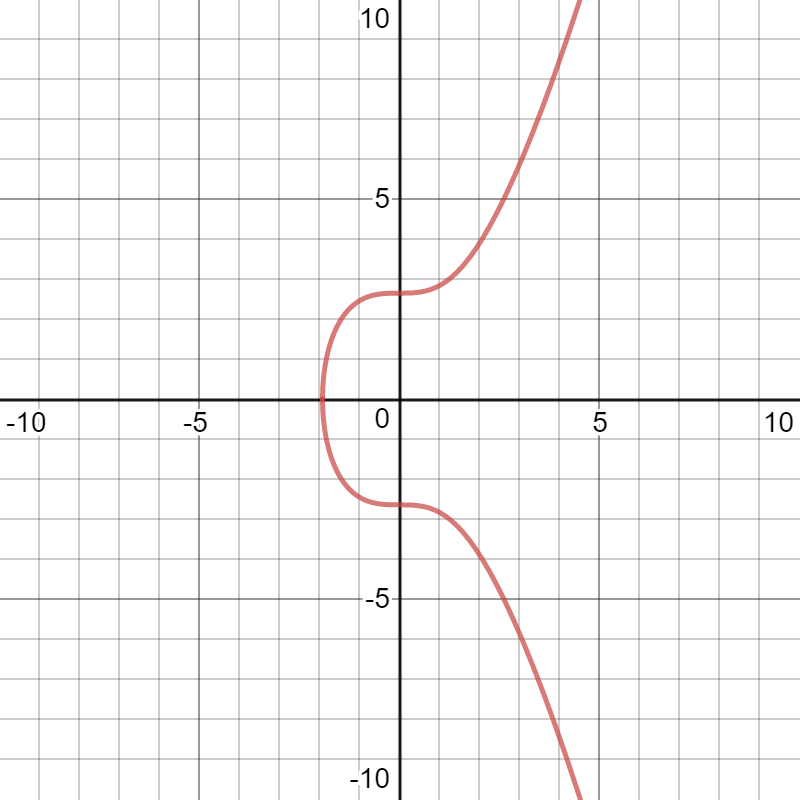
\includegraphics[scale=0.5]{images/ecc.png}
	\caption{Elliptic Curve}
	\label{fig:elliptic_curve}
\end{figure}

Two points are chosen and the public-private key pair is generated using them. The private key is used to sign transactions while the Keccak-256 (A variation of SHA-3) hash of the public key is taken and the rightmost 20 bytes is registered as the Ethereum address.

Addresses in Ethereum are of two types.
\begin{enumerate}
    \item Externally Owned Accounts
    \item Contract Accounts
\end{enumerate}

Externally Owned Accounts are used by nodes to send and receive ether. These are the most commonly used accounts and have an associated private key.

Contract accounts hold the contract code and are used only to execute smart contracts. They do not have an associated private key
\newpage

\subsection{Mining Algorithm}
Ethereum uses Eth-Hash algorithm for finding the cryptographic hash (the process of mining). Before mining starts, a large Directed Acyclic Graph (DAG) is created. The mining process attempts to solve a certain condition in it. This process is the Proof of Work (PoW) in ethereum and is designed to be verified by other nodes very fast in linear time on a CPU using very less resources.

\subsection{Genesis block}
A genesis block is the first block of the entire chain. It is named as block 0.This has to be created manually for private networks and contains a hash of all zeros. In Ethereum, genesis block is represented in the form of a JSON file and is downloaded first when a new node is created and added to an existing Ethereum Network. A sample genesis block is shown below.
\begin{verbatim}
    {
        "nonce": "0x0000000000000042",
        "mixhash": "0x0000000000000000000000000000000000000000000000000000000000000000",
        "difficulty": "0x400",
        "alloc": {}, 
        "coinbase": "0x0000000000000000000000000000000000000000",
        "timestamp": "0x00",
        "parentHash": "0x0000000000000000000000000000000000000000000000000000000000000000",
        "extraData": "0x436861696e536b696c6c732047656e6573697320426c6f636b",
        "gasLimit": "0xffffffff",
        "config": {
            "chainId": 63723,
            "homesteadBlock": 0,
            "eip155Block": 0,
            "eip158Block": 0
        }
    }
\end{verbatim}


\subsection{Crypto-Currency in Ethereum}
Ethereum pays a crypto-currency called ether to successful miners. This can be subdivided into smaller units up to the smallest unit called wei. The name Wei is a tribute to one of the earliest visionaries of cryptocurrency, Wei Dai. He is the author of a protocol and cryptocurrency called b-money \cite{dai1998bmoney}.

Like any other currency, ethereum is not immune from volatility and ranges widely. To prevent volatility in the amount (called gas) that must be paid for executing transactions on the Ethereum network, it is independent from the actual currency. 

Gas can be defined as a special unit used in Ethereum to calculate costs incurred for executing that transaction. Gas limit must be mentioned in the transaction and must be reasonable. If the limit is too low, it is unlikely that any miners will process that transaction. Once the transaction is executed, the miner that processes that transaction will be paid in ether corresponding to the gas that was spent. The remaining gas is returned to the account that requested the transaction.

Table \ref{eth_denominations} shows the different denominations in Ethereum and their exchange rate with ether.

\begin{table}[!htbp]
	\renewcommand{\arraystretch}{1.3}
	\caption{Denominations in Ethereum}
	\label{eth_denominations}
	\centering
	\begin{tabular}{|c||c|c|c|}
		\hline
		\bfseries Name & \bfseries Conversion Rate & \bfseries Special Name & \bfseries In Honor Of\\
		\hline\hline
		$wei$ & $10^{-18}$ & - & Wei Dai \\ \hline
	    $kwei$ & $10^{-15}$ & ada & Ada Lovelace \\ \hline
	    $mwei$ & $10^{-12}$ & babbage & Charles Babbage \\ \hline
	    $gwei$ & $10^{-9}$ & shannon & Claude Shannon \\ \hline
	    $micro$ & $10^{-6}$ & szabo & Nick Szabo \\ \hline
	    $milli$ & $10^{-3}$ & finney & Harold Finney \\ \hline
	    $ether$ & 1 & - & - \\ \hline
	    $kether$ & $10^{3}$ & einstein & Albert Einstein \\ \hline
	    $mether$ & $10^{6}$ & - & - \\ \hline
	    $gether$ & $10^{9}$ & - & - \\ \hline
	    $tether$ & $10^{12}$ & - & - \\ \hline

	\end{tabular}
\end{table}
\newpage
\subsection{Networking Modes in Ethereum}
\subsubsection{Public Network}
There are 2 kinds of public networks run and maintained by the Ethereum network. 
First is the main network with a network id of 1. There are other test networks which can be used by developers to test features of their distributed apps built using ethereum. Table \ref{pub_eth_networks} provides a brief explanation of the different main and test networks. 

\begin{table}[!htbp]
	\renewcommand{\arraystretch}{1.3}
	\caption{Public Ethereum Networks}
	\label{pub_eth_networks}
	\centering
	\begin{tabular}{|c||c|c|c|}
		\hline
		\bfseries Network & \bfseries Type & \bfseries Network ID & \bfseries Network Status \\
		\hline\hline
		$main$ & Main & 1 & Online \\ \hline
		$morden$ & Test & 2 & Retired \\ \hline
		$ropsten$ & Test & 3 & Online \\ \hline
		$rinkeby$ & Test & 4 & Online \\ \hline

	\end{tabular}
\end{table}

\subsection{Private Network}
Private networks can be setup in both closed and open modes. All nodes in this network need to be started with an ID other than the ones used by public networks. Another requirement is that all the nodes in the private network need to be initialized with the same genesis block. A random number \textbf{63723} was chosen for this thesis. If we require that the private network should not be accessed by any one with the network id and genesis block, we can turn off the discovery mode for other peers and instead add them manually.

\subsection{Geth}
An Ethereum node is a client called Geth which is implemented in Golang and is used to connect to the Ethereum network. Other implementations in C++ and Python are also available. Once installed, it can be initiated with a genesis block (the first block in the blockchain), started and connected to different networks available in Ethereum. These networks are identified by their network ID. Since this is a peer to peer protocol, different nodes with the same genesis block and network ID can synchronize with each other and mine transactions. Network ID: 1 is for the main network, 2 and 3 are reserved for Test networks. We can use a different network ID for setting up a private network. Different versions for Windows, Linux, MacOS and Android are available and can be downloaded from the below website.
https://geth.ethereum.org/install/

\begin{table}[!htbp]
	\renewcommand{\arraystretch}{1.3}
	\caption{Example eth and web3 commands in geth}
	\label{geth_commands}
	\centering
	\begin{tabular}{|c|c|c|}
		\hline
		\bfseries API & \bfseries Command & \bfseries Function \\
		\hline\hline
		geth & geth attach & Opens access to blockchain \\ \hline
		eth & eth.coinbase & Address of the primary account \\ \hline
		eth & eth.getBalance() & Returns balance in wei \\ \hline
        eth & eth.sendTransaction() & Sends ether in wei between accounts \\ \hline
        eth & eth.pendingTransactions & Returns list of pending transactions\\ \hline
        eth & eth.coinbase & Address of the primary account \\ \hline
        web3 & web3.fromWei() & Converts wei to Ether \\ \hline
        web3 & eth.toWei() & Converts Ether to wei \\ \hline
        miner & miner.start() & Starts mining on the node \\ \hline
        miner & miner.stop() & Stops mining on the node \\ \hline
        admin & admin.nodeInfo.enode & Gets the ENODE value of the geth node \\ \hline
	\end{tabular}
\end{table}

\newpage
\subsection{Geth Synchronization modes}
Geth can be run in 3 different modes: Full, Fast or light. Each have their own uses and we can setup any node to work in a different mode. 

\subsubsection{Full} 
This is the default mode of geth when run without any synchronization options. It requests the entire state database, gets all the headers, bodies and validates every element from genesis block.

\subsubsection{Fast}
This mode gets the block headers, bodies and doesn't process any transaction until it reaches the current block. Thereafter, it works exactly like a full synchronization.

\subsubsection{Light}
This mode only gets the current state from the blockchain. To verify elements, it needs to request full nodes for the previous states. This is perfect for edge devices like the raspberry pi where we do not want to store much data. However, it requires a full node dedicating some of its resources to serve requests from a light node.

\subsection{Ethereum Virtual Machine}
Ethereum Virtual Machine (EVM) is a virtual environment that runs on all geth nodes and execute the code provided by smart contracts. A variety of programming languages such as Solidity, Vyper, LLL etc are available for writing Contracts which can then be compiled to EVM byte code capable on running in the EVM.

\subsection{Interfacing Methods}
Depending on whether we want to access our node from the same machine or from a different machine on the same or different network, Inter Process Communication (IPC) or Remote Procedure Calls (RPC) may be used.

\subsubsection{Inter Process Communication}
Inter Process Communication (IPC) is the preferred method of connecting to a ethereum node from processes running on the same system. If the node is started without any options, the only method available to connect to the node is through IPC. Geth creates a geth.ipc file in its home directory and must be referenced whenever we want to connect to the system. For security reasons, IPC is limited to localhost and cannot be run from another machine.

\subsubsection{Remote Procedure Calls}
Remote Procedure Calls are to be used if the ethereum node is running on an outside system. Geth provides HTTP as well as WebSocket proxies to connect to ethereum. Additionally, the format used to interface with ethereum is called JSON-RPC. It is the interface using which a front-end application written in any programming language can communicate with the business logic and data stored in the blockchain.

\subsection{Solidity}
Solidity is a Turing complete Contract-oriented programming language available for Ethereum to write Smart contracts. It is a high-level language supporting all features of a modern programming language such as static-typing, inheritance and complex user-defined data types. This enables us to build smart contracts capable of building distributed apps like Maintaining Land ownership records, Voting, Auction and Betting apps among others.

\subsection{Remix}
Smart contracts can be written and tested using a browser-based IDE called Remix. It is available at the below website.
https://remix.ethereum.org

\subsection{Smart Contract}
A smart contract is a Class like code that lives in the Ethereum blockchain (EVM). The methods declared within the smart contract can be run as a transaction by any node which has enough ether to pay for running that transaction. This contract can be accessed by the outside world through distributed apps (also called dapps). Solidity compiler (solc) is used to compile these smart contracts into EVM bytecode (containing machine-code like instructions compiled from solidity) and ABI Definition containing meta-data like the variables and methods used in the smart contract.

A typical Smart Contract consists of variables, setter and getter methods with access modifiers to regulate access exactly like Object-Oriented languages such as C++ and Java. Setter methods involve changing the state of the data contained within in blockchain and thus incur a transaction charge which must be paid in gas. Getter methods only retrieve the data stored within the full node or from a peer and does not incur any charge.

\subsection{Smart Contract Concepts}
A typical Smart Contract looks like a Class definition written in languages like C++ or Java. In addition to commonly available object-oriented principles such as constructors, methods, variables, visibility modifiers, Inheritance, arrays and loops; solidity provides a few additional capabilities to bolster the usability of Smart Contracts for solving several different use-cases.

\subsubsection{solc compiler}
Smart Contracts need to be compiled to EVM byte-code and ABI definition before the Virtual Machine in an ethereum-node can access and execute transactions and methods mentioned in the blockchain. Ethereum tools like Remix and Truffle are bundled with this compiler. The version used to compile the smart contract is mentioned at the very top of the solidity code.

\begin{verbatim}
    pragma solidity ^0.4.24;
\end{verbatim}

0.4.24 is the version of the solidity compiler to be used and the symbol before the version number implies that the source file would not be valid above 0.4.24

\subsubsection{Variables}
Variables in Solidity are statically-typed and must be declared only once. The compiler throws an error if a variable is declared more than once throughout the source file. The table \ref{solidity_data_types} explains some of the commonly used data types available in solidity.
 
\begin{table}[!htbp]
	\renewcommand{\arraystretch}{1.3}
	\caption{Data Types in Solidity}
	\label{solidity_data_types}
	\centering
	\begin{tabular}{|c|c|c|}
		\hline
		\bfseries Data Type & \bfseries Value Types & \bfseries Example \\
		\hline\hline
		boolean & True,False & True \\ \hline
		integer & uint, int & 8, -20 \\ \hline
		address & hexadecimal string & 0x123 \\ \hline
		String & String literals & "foo" \\ \hline
	\end{tabular}
\end{table}

\subsubsection{Arrays}
Arrays can be of dynamic or static lengths. Use of Arrays, either static or dynamic is discouraged in solidity as they can grow to large sizes and require large amounts of gas to process simple operations such as lookup of data.

The below example shows a static array of size 7.
\begin{verbatim}
    uint[] a = new uint[](7);
\end{verbatim}

\subsubsection{Mapping}
Mapping is encouraged to be used within solidity in place of arrays. Mapping is defined as a key value pair of any data types, the key and value part included. They can be thought of as hash tables that are initialized when declared, contain every possible value and are mapped initially to a byte representation of all zeros. The key is not stored in the mapping, only is keccak-256 hash is stored and used to match its corresponding value.

The below example shows how mappings can be declared and used.
\begin{verbatim}
    //declare the mapping
    mapping(address => uint) public balances;
    
    //store value in a mapping
    balances[addressSender] = newBalance;
\end{verbatim}

\subsubsection{Structs}
Structs are similar to the C data type of the same name and are used to typically store the values of a number of related data-items. Structs can be part of the value of a mapping and are used extensively in solidity.

An example struct is shown below
\begin{verbatim}
    //struct to store the temperature, humidity and timeStamp
    struct SensorData{
        uint64 temperature;
        uint64 humidity;
        string dataStorageTime;
    }
    
\end{verbatim}

\subsubsection{Constructor}
Constructors in solidity provide the same functionality as the constructors in any other object oriented programming language. The below example is taken from the smart contract used in this thesis.
\begin{verbatim}
    //Constructor for the Smart Contract
    constructor() public {
        currentID = 1;
        createdBy = msg.sender;
    }
\end{verbatim}

\subsubsection{Methods}
Methods are functions defined within a smart contract and can be used to modify or retrieve the state of the blockchain. However, methods that serve as setters, i.e modify the state of blockchain cannot return an output. Calling such methods from web3 returns only their transaction hashes and gas must be paid in ether for services used. Methods that do not modify the blockchain and simply return the state of a value stored in their local blockchain copy and do not incur any gas costs. Example of a method to set a value.
\begin{verbatim}
    //register IoT device
    function registerDevice(address addressToAdd) ownerOnly public {
        if(devicePresent(addressToAdd)) {
            emit deviceEvent(addressToAdd, "DEVICE ALREADY REGISTERED");
        }
            trustedAddresses[addressToAdd] = true;
            emit deviceEvent(addressToAdd, "SUCESSFULLY REGISTERED");
    }
\end{verbatim}


\subsubsection{Events}
Events are special methods that can be emitted from within a smart contract to indicate a successful transaction or indicate the occurrence of an error. These events can be listened to by another smart contract or from the outside world through web3. An example event is indicated below.
\begin{verbatim}
    //Transaction successful
    event setFileHashEvent(
        address indexed _from,
        string _message
    );
    
    //Event triggered using emit keyword
    emit setFileHashEvent(msg.sender, "FILE HASH TRANSACTION CALLED");
\end{verbatim}


\subsubsection{Modifiers}
Modifiers are used when we want to prevent certain kind of users from accessing the blockchain. A basic form of Access Control can be established within a smart contract using Modifiers. These modifiers can then be applied to methods that are only transacted if the conditions in the modifier are met. Example of a modifier is given below.
\begin{verbatim}
    //Modify some functions to be executed only by the Contract creator
    modifier ownerOnly {
        require(msg.sender == createdBy);
        _;
    }
\end{verbatim}


\subsection{Web3}
Web3 is a framework developed by the Ethereum Foundation which enables a developer to build a client (web application or mobile apps) which can interact directly with the Ethereum Blockchain. Functionality provided by web3 includes getting the wallet address of the current node, sending ether to some other node etc. It can also be used to connect to a Smart Contract which is deployed in the blockchain and run the functions defined in them. These functions can be anything from transferring ownership of land from one person to another person, transferring ether or casting a vote for a candidate in an election. Web3 is available in javascript, python and other languages. Web3.js is by far the most popular framework available which enables us to connect a web page with some functionality to the back-end Smart contract. Most IOT devices have excellent support for C and Python. This is the reason why web3.py was chosen to be used as a interface between IOT devices and the Ethereum Blockchain for this thesis.

\subsection{Truffle}
Truffle is a framework which makes developing and deploying Smart Contracts in Ethereum easier. It can be setup to compile our smart contract and deploy it to our network. Additional functions such as retrieving the smart contract's address and ABI definition can also be done using truffle.

Table \ref{truffle_commands} describes a few commands that allows truffle to compile and deploy smart contracts and Table \ref{truffle_console} provides commands that can run in the truffle console.

\begin{table}[!htbp]
	\renewcommand{\arraystretch}{1.3}
	\caption{Example truffle commands}
	\label{truffle_commands}
	\centering
	\begin{tabular}{|c|c|}
		\hline
		\bfseries Command & \bfseries Function \\
		\hline\hline
		truffle compile & Compiles a smart contract to EVM bytecode \\ \hline
		truffle migrate & Deploys the smart contract to a network mentioned in its configuration \\ \hline
		truffle console & Accesses the meta-data for the smart contract \\ \hline
	\end{tabular}
\end{table}

\begin{table}[!htbp]
	\renewcommand{\arraystretch}{1.3}
	\caption{truffle console commands}
	\label{truffle_console}
	\centering
	\begin{tabular}{|c|c|}
		\hline
		\bfseries Command & \bfseries Function \\
		\hline\hline
		ContractName.address & Returns the address of the Smart Contract \\ \hline
		ContractName.abi & Returns the abi metadata of Smart Contract \\ \hline

	\end{tabular}
\end{table}

\subsection{Ganache}
Ganache is framework which can be useful for testing our smart contract during development. It provides a bootstrapped private blockchain with test accounts with pre-loaded ether.

\section{Alternate Decentralized Storage Solutions}
Ethereum allows data storage via Smart contract variables. However, this will be demonstrated in \ref{chapter:experiment_results} that this storage comes with a steep cost and as the size of the data being stored increased so will the cost to load the transactions to the blockchain.

Another major disadvantage with using Ethereum as the sole data storage mechanism is that the data stored would have to contend with severe limitations placed on the variables by Solidity. This is by design and storing huge volumes of data on blockchain is discouraged by Ethereum to prevent abuse by choking the network causing a Denial of Service for others.

To overcome these limitations, data maybe stored in alternate decentralized storage solutions such as Ethereum Swarm or Inter Planetary File System. We will compare performance using both these solutions in this thesis. Additional storage schemes such as Siacoin, storj etc. are in various stages of development.

\subsection{Ethereum Swarm}
Ethereum Swarm is a storage solution that aims to utilize a bit-torrent like Peer to Peer (P2P) protocol to store data  in a decentralized fashion distributed in a large number of nodes. It is part of the geth tool-chain and uses a lot of technologies invented by the Ethereum foundation. The current implementation is at version 0.3.x or Proof of Concept 3. 

It provides a HTTP proxy to access data stored across nodes. A file stored in Swarm returns a filehash which uniquely identifies that resource.

Its primary objective is to allow dapps to store data efficiently for applications such as messaging, data streaming and mutable resource updates. Since it is endorsed directly by the Ethereum Foundation, swarm makes a pretty good choice in this thesis.


\subsection{Inter Planetary File System}
The Inter Planetary File System (IPFS) is a storage solution, very similar to Ethereum Swarm and solves a lot of the same issues faced by Swarm. However, it has been around for much longer than Ethereum and is much easier to setup and use.

Like Swarm, it returns a filehash for a file stored in the IPFS network. Unlike Ethereum Swarm, it provides a new protocol to access content stored in its nodes.

\subsection{MariaDB}
MariaDB is a fork of the popular MySQL database and is completely maintained by the open source community. It is a relational Database and is used in this thesis to compare performance metrics between a locally stored Database system and the proposed fully distributed storage system.

\subsection{Comparison between Storage Solutions}
\begin{table}[!htbp]
	\renewcommand{\arraystretch}{1.3}
	\caption{Comparison of Swarm and IPFS}
	\label{swarm_eth_comparison}
	\centering
	\begin{tabular}{|c||c|c|c|}
		\hline
		\bfseries Comparison & \bfseries IPFS & \bfseries Swarm & \bfseries RDBMS \\
		\hline\hline
		Decentralization & Yes & Yes & No \\ \hline
		Single Point of Failure & No & No & Yes \\ \hline
		Production Ready & Yes & No & Yes \\ \hline
		Privacy of Data & No & No & Yes \\ \hline
		Speed & Slow & Slow & Fast \\ \hline

	\end{tabular}
\end{table}

\section{IOT Security}
IoT devices are expected to have a huge economic impact in the coming years and is expected to grow exponentially in numbers. This provides a huge incentive for hackers to try and steal sensitive information for sale or other malicious intents. Devices connected to the internet are vulnerable to serious issues if they are not sufficiently protected. Another challenge faced by these edge devices is their weak processing and memory capabilities. We rely on a combination of Public key cryptography, Symmetric encryption and Hashing to transfer keys securely between devices and encrypt and sign telemetry data. 

\subsection{Hardware Security Modules}
Hardware Security Modules such as a Trusted Privacy Module (TPM) are used to help enhance the relatively weak security on a base Raspberry Pi. TPM is used to store important keys in the hardware as well as encrypt the file system and decrypt only while using the device. TPM used in this thesis is called Zymbit 4i, which is an add-on board for the Raspberry Pi and communicates with it via the I2C interface.

\subsubsection{Data Locker keys}
The TPM used, Zymbit 4i, provides a public-private ECDSA key pair for signature generation and verification as well as two keys, one-way and shared. \textbf{One-way} key is used to lock down sensitive files such as secret keys to the machine while the \textbf{shared} key is used to encrypt data saves to Amazon Web Services (AWS) cloud. 

\subsubsection{Linux Unified Key Setup}
The storage medium (SD card is this case) is encrypted fully using LUKS (Linux Unified Key Setup) and dm-crypt. The dm-crypt implementation uses a single Master key to encrypt/decrypt the file system contents shared by several users/ services. Moreover, this single master key needs to be changed frequently to avoid being cracked. This might not always be feasible. LUKS uses a hierarchical key management system to simplify managing keys for each service/user, providing them to services and revoking them when required. However, all these keys are encrypted using the single master key which must be stored on the device storage. Since the SD card can be removed and accessed easily, the master key is at risk of being stolen. The Hardware Security Module/ TPM overcomes this issue by locking the LUKS Master key using its private key stored within the hardware.

\subsection{Cryptography Algorithms used}
\subsubsection{Public Key Cryptography}
Public Key Cryptography uses a key pair of public and private keys to encrypt data as well as provide verification the authenticity of a message.

Ron Rivest, Adi Shamir and Leonard Adleman developed the RSA algorithm which utilizes a public-private key pair to encrypt and decrypt data. It can also be used for verifying signatures. The public key of a recipient is used to encrypt data which can then be used by the recipient to decrypt the data using their private key. Due to payload size constraints, it is typically used to transfer symmetric encryption keys

\subsubsection{Symmetric Encryption}
Symmetric Encryption uses a single secret key to encrypt and decrypt data. Symmetric key encryption is used to encrypt or decrypt huge volumes of data and is generally faster than Public Key Cryptography. The downside is that the secret key must be stored safely and must be changed frequently.

Advanced Encryption Standard (AES) utilizes a strong secret key to encrypt actual data. We use this algorithm to encrypt and store data in Swarm or IPFS. Since the system we are proposing requires many devices sharing the same key, using public key cryptography was considered for this thesis.  
\subsubsection{Hashing}
Hashing is the process of generating a set of characters that can uniquely identify a particular input. In Cryptography, they are used mainly to generate a signature for a larger input and encrypt it with a sender's private key, and can be decrypted only using the sender's public key. This authenticates the data received as only the sender's public key can decrypt data encrypted using its private key pair. Secure Hashing Algorithms (SHA series), Message Digest (MD series) and Hash Message Authentication Code (HMAC) are some of the hashing algorithms in popular use.

A hash algorithm (HMAC) is used in this thesis to sign the un-encrypted payload and is used to verify the authenticity and data integrity of the message. 



\chapter{Methodology} \label{chapter:proposed_system}

\section{High-level Design} \label{ss:construct_architecture}
The proposed system explained in \ref{fig:impldiagram_architechture} consists of number of applications running on a Local machine (miner nodes) whose sole purpose is to validate the transactions called by the set methods in the smart contract. One of the raspberry pis, called IoT Producer will be used to gather readings. The IoT producer will be running geth in light mode, swarm and ipfs applications to send data to rest of the network. The other raspberry pi, called IoT consumer will be used to get the readings from the network and use them to send out the data to other end-points such as APIs or LCD displays. The connections between the Producer and Consumer isn't rigid and each connect to the Ethereum, Swarm or IPFS network.

\begin{figure}
	\centering
	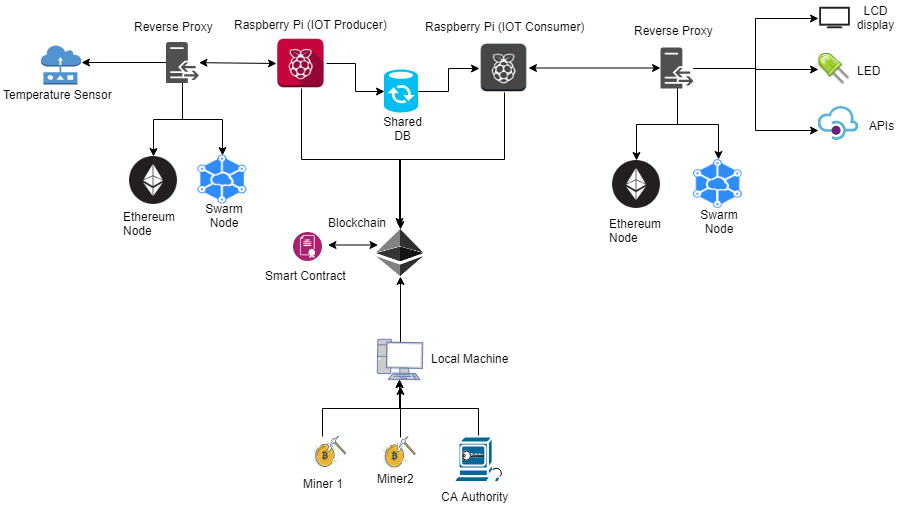
\includegraphics[scale=0.5]{images/Final_Implementation.png}
	\caption{Implementation Diagram}
	\label{fig:impldiagram_architechture}
\end{figure}


\section{Proposed System Components}
This section explains in detail, the different systems working together to achieve the expected results.

\subsection{Local Machine}
The test machine validating the mining operations is a laptop with Core i7-7700HQ processor rated at 2.8GHz with 4 physical cores and 16 GB RAM. This machine runs two geth miner nodes (for redundancy). One of the miner nodes dedicates a few of its resources to serve requests from light geth nodes.

\subsection{IoT Edge Nodes}
We will setup two identical Raspberry Pis, each serving different purposes. One of the raspberry pi's will be used to read telemetry data from sensors while the other will be used to output this data to a display device or the console.
The raspberry pi model used is a Raspberry Pi 3 Model B with a 1.2 GHZ quad-core ARM Cortex A53 processor with 1 GB DDR2 RAM. A 32GB class 10 SD card encrypted by LUKS and dm-crypt serves as the storage medium. Raspbian Stretch Lite is flashed onto both the nodes and booted up.

\subsubsection{IoT Producer}
The IoT Producer is used to read data from all the sensors, encrypt and store data in the decentralized network. The geth node running in this machine is a light node which depends on a mining node to get full information about the blocks in the chain. Ethereum is merely used to store references to the data collected by the system. It is setup to be able to connect to instances of either swarm or IPFS, or even run its own instances, depending on our selection and store the actual data in encrypted form.

For testing and demo purposes, a Digital Humidity and Temperature Sensor (DHT11) is attached to the raspberry pi to GPIO 22 pin for data, xx for voltage and yy ground pin.

\subsubsection{IoT Consumer}
The IoT Consumer is used for demonstration purposes in this thesis. Like the IoT Producer, it connects to or runs instances of IPFS or Swarm and runs a light version of geth. It retrieves the reference from the Ethereum blockchain and requests the correct information from swarm or IPFS.

Two IoT devices are connected to the consumer for testing and demo purposes, the first is a 3 color LED which is connected to GPIO xx,yy and zz pins of the consumer and a ground pin connected to pin ww. The second device is a I2C LCD which is connected to the SDA1(XX) and SCL1(yy) pins for I2C bus, 3.3V (zz) for power and ww ground pin.


\section{Software Setup}
Python3 is used to write scripts that interface with IoT devices, Ethereum blockchain, IPFS and Swarm. Its package manager pip3 is installed in all the devices we use. The environment used in our test devices are tabulated in \ref{environment_setup}. Node.js with its package manager npm, is used to build, compile and deploy Solidity based Smart Contracts. 

\begin{table}[!htbp]
	\renewcommand{\arraystretch}{1}
	\caption{Environment Setup}
	\label{environment_setup}
	\centering
	\begin{tabular}{|c|c|c|c|c|c|}
		\hline
		\bfseries Device & \bfseries OS & \bfseries Architecture & \bfseries Python Version & \bfseries Node.js & \bfseries Solidity\\
		\hline\hline
		$Local Machine$ & Ubuntu 18.10 & amd64 & Python 3.5 &  Yes & Yes\\ \hline
		$IoT Producer$ & Raspbian Stretch Lite & armv7 & Python 3.5 &  No & No\\ \hline
		$IoT Consumer$ & Raspbian Stretch Lite & armv7 & Python 3.5 &  No & No\\ \hline
	\end{tabular}
\end{table}

\subsection{Software binaries}
Pre-built Geth binaries are downloaded for the local machine(amd64) as well as the IoT nodes(arm). Ethereum-Swarm packages are readily available for Ubuntu but not easily available for the Raspberry Pi 3.
Raspberry pi 3B doesn't have the capabilities to build these binaries from source. 
Fortunately, Geth and swarm were built using the Go programming language which provides excellent cross-compilation tools. The local machine was used to build the swarm binary and these binaries were installed on the raspberry pis. Table \ref{software_version} provides information on the different versions of geth, swarm and IPFS used in this thesis.

\begin{table}[!htbp]
	\renewcommand{\arraystretch}{1}
	\caption{Software binary versions}
	\label{software_version}
	\centering
	\begin{tabular}{|c|c|c|c|}
		\hline
		\bfseries Device & \bfseries Geth & \bfseries Swarm  & \bfseries IPFS\\
		\hline\hline
		$Local Machine$ & 1.8.23-stable & 0.3.11-stable & 0.4.19 \\ \hline
		$IoT Producer$ & 1.8.23-stable & 1.6.7-stable & 0.4.19 \\ \hline
		$IoT Consumer$ & 1.8.23-stable & 1.6.7-stable & 0.4.19 \\ \hline
	\end{tabular}
\end{table}

\subsection{Python modules}
Since python3 is used extensively, a couple of third party python modules are used to help with accessing the blockchain, write data to ipfs or encrypt and decrypt data. Table \ref{python_modules} describes all the modules used in this thesis.
\begin{table}[!htbp]
	\renewcommand{\arraystretch}{1.3}
	\caption{Third party Python modules}
	\label{python_modules}
	\centering
	\begin{tabular}{|c|c|c|}
		\hline
		\bfseries Module Category & \bfseries Module Name & \bfseries Usage \\
		\hline\hline
		$Storage$ & web3 & To access smart contract functions or get balances \\ \hline
		$Storage$ & ipfsapi & To store and retrieve data from IPFS \\ \hline
		$IoT$ & AdafruitDHT & Get temperature, humidity from DHT \\ \hline
		$Cryptography$ & pycryptodomex & Implementations of Cryptography algorithms \\ \hline
	\end{tabular}
\end{table}



\section{IoT Security Considerations}
\subsection{Hardware Security}
A Trusted Privacy Module device, Zymbit 4i is used as a Hardware Security mechanism for the raspberry pi. It occupies the first 10 GPIO pins, including one 3.3V pin, 2 5V pins, 2 Ground pins, GP104 and the I2C bus. Before installing it, the I2C interfacing option is first activated on the Raspberry Pi. Finally, the required software modules needed for accessing the hardware keys stored on the TPM device are installed. Once this setup is completed, the root file system is encrypted using LUKS and dm-crypt using the private hardware key stored on the TPM.

\subsubsection{Boot Sequence of normal LUKS}
\begin{enumerate}
	\item Kernel initializes initramfs - A single cpio archive loaded into main memory during startup
	\item initramfs presents decryption key to LUKS
	\item LUKS decrypts the root file system
\end{enumerate}

There are a couple of issues with the above procedure when Raspberry Pi is involved. First is that there is no dedicated key-ring for storing cryptographic keys available in other Operating Systems. Secondly, the decryption key should not be stored in plain text on the removable SD card. To fix these issues, a TPM is used with LUKS for a more secure boot sequence.

\subsubsection{Boot Sequence of LUKS with TPM}
\begin{enumerate}
	\item Kernel initializes initramfs
	\item initramfs present locked LUKS key to TPM
	\item TPM verifies the key signature and decrypts the LUKS key
	\item Unlocked LUKS key is used to decrypt the root file system
\end{enumerate}

\subsection{Software Security}
\subsubsection{Change default password}
The default password on the raspberry pi is \textbf{raspberry}. According to a research \cite{8364059}, IoT devices are easily hacked due to improper setup, often times leaving the default credentials in place. The first priority after setting up the raspberry pi must be to change the password to something more secure.

\subsubsection{Replace default user}
To further increase security, a new user is added and the default \textbf{pi} is deleted. Another feature to consider is to request the password when a terminal runs a \textbf{sudo} command which is turned off in raspbian by default.

\subsubsection{Installing Firewall}
There is no firewall installed by default on the raspberry pi. Uncomplicated Firewall (ufw) can be setup very easily in any linux based OS and the raspbian OS is no different. All ports except for those we need such those for making remote procedure calls, networking between geth, swarm or ipfs nodes are selectively enabled.

\subsubsection{Transferring Symmetric keys}
Symmetric keys must never be transferred in plain-text format over network or stored in the file system in plain text. The below sequence of steps are used to transfer AES keys over a network and lock them to the raspberry pi.

\begin{enumerate}
	\item Generate RSA public - private key pair on Raspberry Pi
	\item Transfer public key over to host machine generating symmetric key using a secure channel such as Secure Copy (scp) or Secure File Transfer Protocol (sftp)
	\item Generate a signature hash for the key
	\item Encrypt the symmetric key with the raspberry pi's public key
	\item Transfer the encrypted symmetric key back to the raspberry pi
	\item Decrypt the symmetric key using the raspberry pi's private key
	\item Verify the signature from the decrypted text
	\item Once signature is verified, use the one-way key from TPM to encrypt and store the symmetric key, which is only decrypted, used and discarded when data collection script starts
\end{enumerate}

\section{Payload Format} \label{ss:payload format}
The payload stored in the storage systems from the sensors can be modified at will, and is independent of the data format enforced by the blockchain. It also allows data to be encrypted before storage. Payload is generated and stored in JSON format as referenced in Table \ref{payload_format}. All values are stored as strings and then formatted into either integer, floating-point numbers or timestamp when needed.
\newpage

\begin{table}[!htbp]
	\renewcommand{\arraystretch}{1.3}
	\caption{Payload Format}
	\label{payload_format}
	\centering
	\begin{tabular}{|c|c|c|c|}
		\hline
		\bfseries S.No & \bfseries Payload Item & \bfseries Brief Explanation & \bfseries Example Data \\
		\hline\hline
		$1$ & Temperature & Temperature collected from sensor in C & 23 \\ \hline
		$2$ & Humidity & Humidity collection from the sensor in \% & 44 \\ \hline
		$3$ & Temperature Units & Units used for temperature (C or F) & F \\ \hline
		$4$ & Humidity Units & Units used for humidity & \% \\ \hline
		$6$ & Timestamp & Time stamp of data collection & 2019-03-13 22:06:09 \\ \hline
		$6$ & Device ID & IoT device ID & IoTProducer1 \\ \hline
		$7$ & Device Type & IoT device type & RaspberryPi3 B \\ \hline
		$8$ & Device IP & IP of IoT device& 192.168.0.16 \\ \hline
		$9$ & Sensor Type & Type of the Sensor Used & DHT11 \\ \hline
	\end{tabular}
\end{table}

\section{Data Flow}
The steps to collect and retrieve the sensor data after applying encryption, verification or decryption.

\begin{figure}
	\centering
	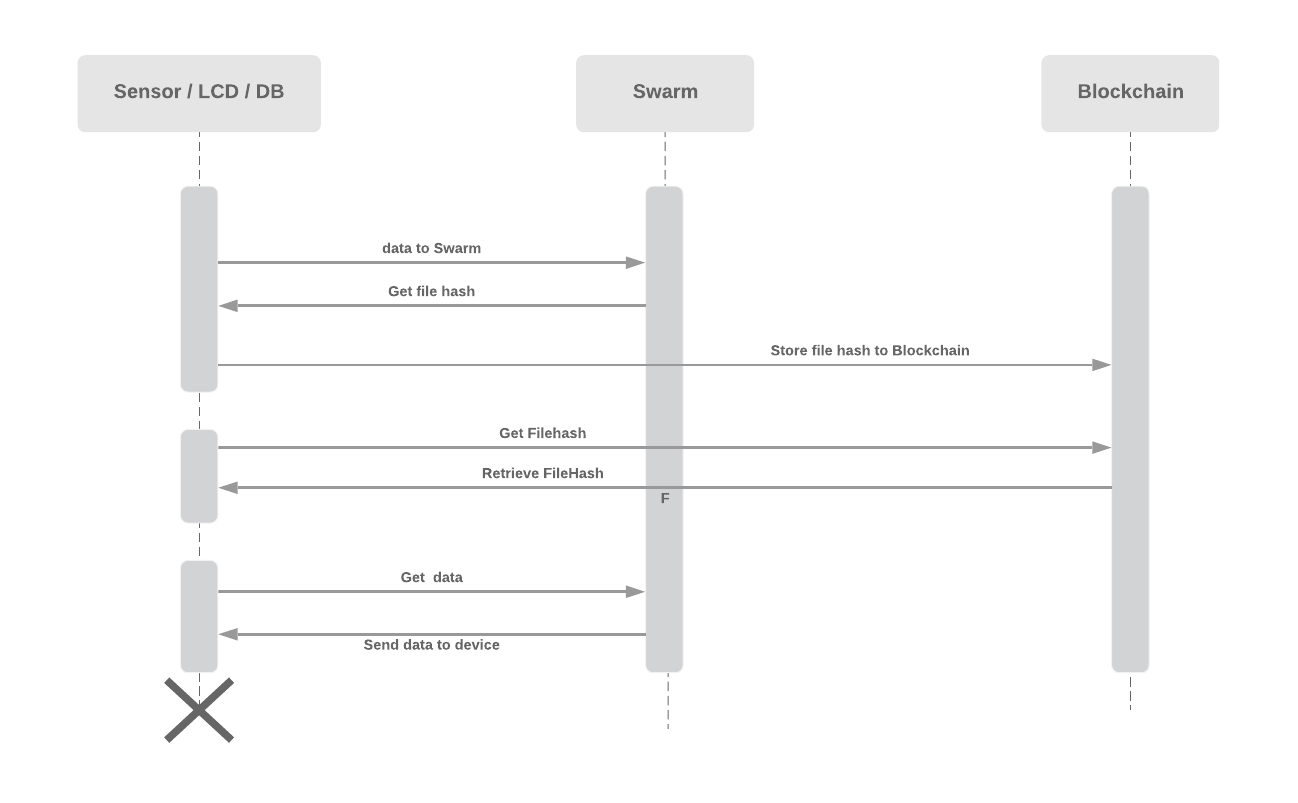
\includegraphics[scale=0.75]{images/DataFlow.png}
	\caption{Data Flow Diagram}
	\label{fig:dataflow_diagram}
\end{figure}

\subsection{Sensor Data Collection}
The Algorithm \ref{alg:data_collection} explains the overall steps followed on the Producer side to collect data from the sensor, sign and encrypt it. The data is then saved to IPFS or Swarm and the resulting filehash is stored in Ethereum.
\newpage
\begin{algorithm}[Data Collection and Payload Storage]
 \KwData{TPM Private key $tpmPrivKey$, Encrypted AES key $cipherText$}
 \KwResult{ Collect and Encrypt Payload, Store in Swarm or IPFS }
  secretKeyAES = decrypt($tpmPrivKey$,$cipherText$)\;
  //Run indefinitely \newline
 \While{True}{
  temperature, humidity =  dataCollectionFromSensor()\;
  timestamp = getCurrentTime()\;
  payload = buildPayload(temperature,humidity,timestamp)\;
  signature = generateSHA256(payload)\;
  payloadCipher = encrypt(secretKeyAES,payload,signature)\;
  filehash = setSwarmOrIPFSData(payloadCipher)\;
  callSetFileHashSensorContract(filehash)\;
 }
 \caption{Data Collection and Payload Storage}
 \label{alg:data_collection}
\end{algorithm}

\subsection{Sensor Data Retrieval}
The Algorithm \ref{alg:data_retrieval} explains the steps followed on the Consumer side to retrieve file-hashes from Ethereum and using it to get the encrypted payload from Swarm or IPFS, decrypt and verify the signature of the payload.

\begin{algorithm}[Data Retrieval and Use]
 \KwData{TPM Private key $tpmPrivKey$, Encrypted AES key $cipherText$}
 \KwResult{ Retrieve Encrypted Payload from Swarm or IPFS }
  secretKeyAES = decrypt($tpmPrivKey$,$cipherText$)\;
  //Run indefinitely \newline
 \While{True}{
    filehash = callGetLatestFileHash()\;
    payloadCipherText = getSwarmOrIPFSData(filehash)\;
    payloadPlainText, signature = decrypt(secretKeyAES, payloadCipherText)\;
    \eIf{generateSHA256(payloadPlainText) == signature}{
        Send to other sources\;
    }{
        Throw Signature Not Verified Error\;
    }
 }
 \caption{Data Retrieval and Use}
 \label{alg:data_retrieval}
\end{algorithm}

\section{Smart Contract Logic Functions}
This section details our logic used within the smart contract to define access control, store and retrieve file-hashes for payload loaded to IPFS or Swarm. 

\subsection{struct to store the collected data}
Although only filehash is part of the struct, it was left in place for future enhancements, if needed.
\begin{verbatim}
    //struct to store the file-hashes which store the actual sensor data
    struct SensorData{
        //filehash is the swarm handle containing the actual sensor readings
        string filehash;
    }
\end{verbatim}

A previous version of the struct in Smart contract when everything was stored on the blockchain, was written as shown.

\begin{verbatim}
    //struct to store the temperature, humidity and time when reading occurred
    struct SensorData{
        uint64 temperature;
        uint64 humidity;
        string dataStorageTime;
    }
\end{verbatim}

\subsection{pointer to data}
An integer value, ID is used as a pointer to refer to our current readings stored/ retrieved by the smart contract.
\begin{verbatim}
    uint public currentID;
\end{verbatim}

\subsection{pointer to data}
An integer value, ID is used as a pointer to refer to our current readings stored/ retrieved by the smart contract.
\begin{verbatim}
    uint public currentID;
\end{verbatim}

\subsection{Mapping from pointer to struct and addresses registered}
The mapping \textbf{sensorDataStore} from ID to SensorData struct is stored. Another mapping stores the registered addresses that are allowed to write or read data to the system.
\begin{verbatim}
    //map the struct to an id
    mapping(uint => SensorData) sensorDataStore;

    //store registered addresses in mapping
    mapping (address => bool) private trustedAddresses;
\end{verbatim}

\subsection{Constructor to initialize the ID}
The ID must be initialized before access and so a constructor is used for this purpose. \textbf{1}  is chosen as the start index. Another variable, createdBy is used to store the contract owner and will be responsible for registering and de-registering IoT devices to the system.
\begin{verbatim}
    //Contract created by
    address private createdBy;
    //Constructor for the Smart Contract
    constructor() public {
        currentID = 1;
        createdBy = msg.sender;
    }
\end{verbatim}

\subsection{Modifier to only allow owner to register and de-register ids}
Access to certain Contract methods such as register or de-registering devices must be held only by the administrator. In this case, the contract creator is the admin and so only the address that created the contract is allowed to run methods which enforce the ownerOnly modifier.
\begin{verbatim}
    //Modify some functions to be executed only by the Contract creator
    modifier ownerOnly {
        require(msg.sender == createdBy);
        _;
    }
\end{verbatim}

\subsection{Events to log Registration and Changing State}
As explained earlier in Chapter \ref{chapter:background}, transactions aren't capable of returning an output value. So we use events that are emitted in response to certain conditions that occur while a transaction is being executed.

\begin{verbatim}
    //event after registration/de-registration
    event deviceEvent(
        address indexed _from,
        string _message
    );
    
    //event after registration/de-registration
    event setFileHashEvent(
        address indexed _from,
        string _message
    );
\end{verbatim}

\subsection{Function to get the current ID}
This method describes how to return the currentID being used to load data to the system.
\begin{verbatim}
    //function to get the currentID
    function getCurrentID() public view returns(uint){
        return currentID;
    }
\end{verbatim}
\subsection{Function to increment the current ID}
This method describes how to increment the currentID being used to load data to the system.
\begin{verbatim}
    //function to increment the ID used internally for managing file-hashes
    function incrCurrentID() public{
        currentID++;
    }
\end{verbatim}

\subsection{Function to set the SensorData filehash}
This method is used to initiate a transaction to add a new filehash received from the storage system and save it to the mapping we have declared earlier. If the device is not registered, an event with the appropriate message is emitted. On success, another event is triggered which relays that the transaction was successful to all the listeners.

\begin{verbatim}
    //Function to store the filehash from swarm
    function setSensorData(string _filehash) public {
        if(devicePresent(msg.sender)) {
            uint idToStore = getCurrentID();
            SensorData storage sensorReadings = sensorDataStore[idToStore];

            sensorReadings.filehash = _filehash;
       
            incrCurrentID();
            
            emit setFileHashEvent(msg.sender, "FILE HASH TRANSACTION CALLED");
        } else {
            emit setFileHashEvent(msg.sender, "DEVICE NOT REGISTERED");
        }
    }
\end{verbatim}

\subsection{Function to get the latest SensorData filehash}
This function returns the latest filehash stored in the blockchain. Using the currentID variable declared earlier, we retrieve the value of the key, currentID from the sensorDataStore mapping.

\begin{verbatim}
    //Function to get the latest stored data
    function getSensorDataLatest() public view returns (string){
        if(devicePresent(msg.sender)) {
            SensorData storage sensorReadings = sensorDataStore[getCurrentID()-1];

            return sensorReadings.filehash;
        }
        return "DEVICE NOT REGISTERED";
    }
\end{verbatim}

\subsection{Function to get the SensorData filehash from any ID}
This method works in a similar fashion to the above method, but retrieves the value associated with the given ID from the sensorDataStore mapping.

\begin{verbatim}
    //Function to get the data stored under some ID
    function getSensorDataByID(uint ID) public view returns (string){
        if(devicePresent(msg.sender)) {
            SensorData storage sensorReadings = sensorDataStore[ID];

            return sensorReadings.filehash;
        }
        return "DEVICE NOT REGISTERED";
    }
\end{verbatim}

\subsection{Methods to register and deregister IoT devices}
The following methods explain how to check if the device is registered and call register or deregister methods for any device and can be only accessed by the contract owner. 
The method "devicePresent" returns if the device is registered with the system.
The methods "registerDevice" and "deregisterDevice" are used to 
\begin{verbatim}
    //function to check if device is registered
    function devicePresent(address addressToAdd) public view returns (bool) {
            return trustedAddresses[addressToAdd];
    }
    
    //register IoT device
    function registerDevice(address addressToAdd) ownerOnly public {
        if(devicePresent(addressToAdd)) {
            emit deviceEvent(addressToAdd, "DEVICE ALREADY REGISTERED");
        }
            trustedAddresses[addressToAdd] = true;
            emit deviceEvent(addressToAdd, "SUCESSFULLY REGISTERED");
    }
    
    
    //deregister IoT device
    function deregisterDevice(address addressToRemove) ownerOnly public {
        if(!devicePresent(addressToRemove)) {
            emit deviceEvent(addressToRemove, "DEVICE NOT REGISTERED");
        }
            trustedAddresses[addressToRemove] = false;
            emit deviceEvent(addressToRemove, "SUCESSFULLY DEREGISTERED");
    }
\end{verbatim}
\newpage

\section{IPFS or Swarm Logic}

For IPFS or Swarm, we will be using the provided HTTP proxy to store and retrieve the payload. Since we are using python, the requests module came in handy to send POST and GET requests from the storage systems. Storing the data then boils down to a simple POST request as explained in Algorithm \ref{alg:payload_storage}.

\begin{algorithm}[setSwarmOrIPFSData]
 \KwData{Encrypted and Signed Payload $encryptedPayload$}
 \KwResult{ Return File hash $filehash$ from IPFS or Swarm }
  result = sendHTTPPostRequest("HTTPProxyEndpoint", data=$encryptedPayload$, headers={'Content-Type': 'text/plain'})\;
  filehash = result.text\;
 \caption{Payload Storage in IPFS or Swarm}
 \label{alg:payload_storage}
\end{algorithm}

A GET request retrieves the payload from the system using the filehash as input which is explained in Algorithm \ref{alg:payload_retrieval}.

\begin{algorithm}[getSwarmOrIPFSData]
 \KwData{File hash of Payload $filehash$}
 \KwResult{ Return Encrypted and Signed Payload $encryptedPayload$ }
  result = sendHttpGETRequest("HTTPProxyEndpoint" + $filehash$)\;
  $encryptedPayload$ = result.text\;
 \caption{Payload Retrieval from IPFS or Swarm}
 \label{alg:payload_retrieval}
\end{algorithm}



\section{Evaluation Methods}
Once the network is setup, performance of the system will be tested in terms of Transactions per Second (TPS), cost per transaction, CPU and memory usage.

\subsection{Ethereum}
To test Ethereum, the primary parameters can be measured for both the filehash and full payload. The primary accounts in all the nodes of the system are transferred 100 Ethereum each to perform these experiments. 
\begin{enumerate}
    \item Cost incurred per transaction
    \item Time taken to transact Set Data method
    \item Time taken to retrieve per record
    \item CPU and RAM usage
    \item Difficulty
    \item Gas Limit and Spending
    \item Transactions per block
    \item Average block creation time
    \item Average Network Hashrate
\end{enumerate}
The network can be fine-tuned to include more transactions per block by adjusting gas limit per transaction.

\subsection{IPFS and Swarm}
Testing IPFS and Swarm can be done using similar means. The below parameters are considered during testing their individual performance on the proposed system.

\begin{enumerate}
    \item Time taken to insert one payload record
    \item Time taken to retrieve one payload record
    \item CPU and RAM usage
\end{enumerate}

\subsection{Data Collection For testing performance}
\subsubsection{Real-time data}

\subsubsection{Simulated data}



%To main things in \LaTeX should be labelled: Figures and Tables.
%
%\section{Figures}
%
%The file {\tt unlv\_macros.tex} contains a number of spiffy macros to
%make figures for you. For example, Fig.~\ref{fig:fancy} is generated
%by the
%command:\\ \verb+\DoFigure{radiusball}{0.5}{This is a fancy picture}{fig:fancy}+. The
%command takes in 4 arguments: the pdf file's name (without .pdf), the
%scaling factor, the caption and the label name (which you can later
%use to refer to the figure's number.)
%
%\DoFigure{radiusball}{0.5}{This is a fancy picture}{fig:fancy}
%
%\newpage 
%\noindent
%We could have built the same directly (see Fig.~\ref{fig:fancy2}) like this:\\
%
%\noindent
%\verb+\begin{figure}[htb!]+\\
%\verb+\begin{center}+\\
%\verb+\includegraphics[scale=0.5]{radiusball}+\\
%\verb+\caption{This is a fancy picture again.}\label{fig:fancy2}+\\
%\verb+\end{center}+\\
%\verb+\end{figure}}+\\
%
%
%\begin{figure}[htb!]
%\begin{center}
%\includegraphics[scale=0.5]{radiusball}
%\caption{This is a fancy picture again.}\label{fig:fancy2}
%\end{center}
%\end{figure}
%
%The macro package also contains macros for double pictures:
%
%\DoBiFigure{radiusball}{radiusball}{0.4}{A shared caption for the pictures.}{fig:double}
%
%or for double pictures with separate captions:
%
%\DoDiFigure{radiusball}{0.4}{A caption for the left pictures.}{fig:di1}{radiusball}{0.4}{A caption for the right pictures.}{fig:di2}
%
%\section{Tables}
%
%A table is most easily made with the {\tt tabular} environment. This environment can 
%produce {\it very} fancy tables, so you might need to go look it up on the web.
%
%\begin{table}[!htb]
%\begin{center}
%\begin{tabular}{||c|l|r||} \hline
%Column 1 & Column 2 & Column 3 \\ \hline\hline
%Foo & 1\" & 2.54cm\\
%Bar & 2\" & 6.08cm\\ \hline
%Baz & \multicolumn{2}{|c||}{Who knows?} \\ \hline
%\end{tabular}
%\caption{A table!}\label{tab:atable}
%\end{center}
%\end{table}

\chapter{Experimental Results}
\label{chapter:experiment_results}
We will test both cost incurred by the account calling the transactions and time taken with and without encryption.


\section{Datasets}
4 datasets
collected
simulated for 1000, 10k and 100k records

\section{Cost Comparison}
\subsection{Data stored in Ethereum}
\subsection{Data stored in Ethereum and Swarm}
\subsection{Data stored in Ethereum and IPFS}
\subsection{Comparisons between different methods}

\section{Performance Comparison}
\subsection{Data stored in Ethereum}
\subsection{Data stored in Ethereum and Swarm}
\subsection{Data stored in Ethereum and IPFS}
\subsection{Comparisons between different methods}


\chapter{Conclusion and Future Work} \label{chapter:conclusion}
\section{Conclusion}


\section{Future Work}
The next areas of focus would be to enhance the quality and types of Sensor data stored and retrieved, secure the IoT devices even further and develop a faster Proof of Work algorithm to validate transactions on the Ethereum blockchain. 

A major area of improvement would be to allow multiple producers to send their sensor data to a single time-stamped Swarm link between time intervals. This would allow for much easier processing of data collected from differed sources.

Another area of improvement from a blockchain perspective is to use a permissioned blockchain like Quorum instead of a open blockchain like Ethereum run in private mode. This allows for much better Access Control and permission for users.

IoT devices are usually under powered due to power usage limitations. Using resource heavy encryption like RSA and AES (even with hardware acceleration) on these edge devices is counter-intuitive to the idea of low power devices dedicated for sensing and collecting data. Modern encryption methods like Adiantum \cite{DBLP:journals/tosc/CrowleyB18} are tailored for low powered edge nodes and are slowly gaining momentum. Early tests with this algorithm has been promising in terms of resource utilization and speeds.

A fast Proof of Work algorithm could be developed as an aim with the express purpose of developing an algorithm for achieving Consensus which is more suitable for IoT data than that is used currently to approve crypto-currency transactions. This optimization would make the algorithm much faster as the complexity of the smart contract increases.


%%%
%%% The bibliography - you can change the alpha to suit your style if you don't like it is it is.
%%% The bib file should be called 'thesis.bib' - if not then change the second line here to be correct.
\bibliographystyle{alpha}
\thesisbibliography{thesis}


%%%
%%% Vita comes next
\vita
\chapter{} %% please leave this one blank - the vita stuff is sort of a hack.
\linespread{1.3} 
\begin{center}
Graduate College\\
University of Nevada, Las Vegas\\[1cm]
Vinay Kumar Calastry Ramesh\\[1cm]
\end{center}

\noindent Degrees:\\
\indent Bachelor of Technology in Computer Science 2014\\
\indent Jawaharlal Nehru Technological University, Hyderabad, India\\

\noindent Thesis Title: Secure Decentralized Storage Using Blockchain\\

\noindent Thesis Examination Committee:\\
\indent Chairperson, Dr. Yoohwan Kim, Ph.D.\\
\indent Committee Member, PUT COMMITTE MEMBER HERE\\
\indent Committee Member, PUT COMMITTE MEMBER HERE\\
\indent Graduate Faculty Representative, PUT COMMITTE MEMBER HERE\\

\end{document}





